% %%%%%%%%%%%%%%%%%%%%%%%%%%%%%%%%%%%%%%%%%%%%%%%%%%%%%%%%%%%%%%%%%%%
% \documentclass[12pt]{article}
% \usepackage{amsmath}
% \usepackage{amsfonts}   % if you want the fonts
% \usepackage{amssymb}    % if you want extra symbols
% \usepackage{graphicx}   % need for figures
% \usepackage{xcolor}
% \usepackage{bm}
% \usepackage{secdot}		
% \usepackage{mathptmx}
% \usepackage{float}
% \usepackage[utf8]{inputenc}
% \usepackage{textcomp}


% \usepackage[hang,flushmargin,bottom]{footmisc} % footnote format

% \usepackage{titlesec}
% \titleformat{\section}{\normalsize\bfseries}{\thesection.}{1em}{}	% required for heading numbering style
% \titleformat*{\subsection}{\normalsize\bfseries}

% \usepackage{tocloft}	% change typeset, titles, and format list of appendices/figures/tables
% \renewcommand{\cftdot}{}	
% \renewcommand{\contentsname}{Table of Contents}
% \renewcommand{\cftpartleader}{\cftdotfill{\cftdotsep}} % for parts
% \renewcommand{\cftsecleader}{\cftdotfill{\cftdotsep}}
% \renewcommand\cftbeforesecskip{\setlength{4pt}{}}
% \addtolength{\cftfignumwidth}{1em}
% \renewcommand{\cftfigpresnum}{\figurename\ }
% \addtolength{\cfttabnumwidth}{1em}
% \renewcommand{\cfttabpresnum}{\tablename\ }
% \setlength{\cfttabindent}{0in}    %% adjust as you like
% \setlength{\cftfigindent}{0in} 

% %% For Tables 
% % \setlength{\arrayrulewidth}{1mm}
% % \setlength{\tabcolsep}{10pt}
% \renewcommand{\arraystretch}{1.5}
%%%%%%%%%%%%%%%%%%%%%%%%%%%%%%%%%%%%%%%%%%%%%%%%%%%%%%%%%%%%%%%%%%%
\documentclass[12pt]{article}
\usepackage{amsmath}
\usepackage{amsfonts}   % if you want the fonts
\usepackage{amssymb}    % if you want extra symbols
\usepackage{graphicx}   % need for figures
\usepackage{microtype}
\usepackage{subfig}
\usepackage{eurosym}
\usepackage{siunitx}
\usepackage{xcolor}
\usepackage{bm}
\usepackage{secdot}		
\usepackage{mathptmx}
\usepackage{float}
\usepackage[utf8]{inputenc}
\usepackage{textcomp}
\usepackage{longtable}
\usepackage[hang,flushmargin,bottom]{footmisc} % footnote format
\usepackage{minted}
\usepackage{titlesec}
\setcounter{tocdepth}{5}
\setcounter{secnumdepth}{5}
\titleformat{\section}{\normalsize\bfseries}{\thesection.}{1em}{}	% required for heading numbering style
\titleformat*{\subsection}{\normalsize\bfseries}
\usepackage{adjustbox}
\usepackage{tocloft}	% change typeset, titles, and format list of appendices/figures/tables
\renewcommand{\cftdot}{}	
\renewcommand{\contentsname}{Table of Contents}
\renewcommand{\cftpartleader}{\cftdotfill{\cftdotsep}} % for parts
\renewcommand{\cftsecleader}{\cftdotfill{\cftdotsep}}
% \renewcommand\cftbeforesecskip{\setlength{4pt}{}}
\addtolength{\cftfignumwidth}{1em}
\renewcommand{\cftfigpresnum}{\figurename\ }
\addtolength{\cfttabnumwidth}{1em}
\renewcommand{\cfttabpresnum}{\tablename\ }
\setlength{\cfttabindent}{0in}    %% adjust as you like
\setlength{\cftfigindent}{0in} 
\cftsetindents{table}{1em}{5em}
%% For Tables 
% \setlength{\arrayrulewidth}{1mm}
% \setlength{\tabcolsep}{10pt}
\renewcommand{\arraystretch}{1.5}



\usepackage{enumitem}         % to control spacing between bullets/numbered lists

\usepackage[numbers,sort&compress]{natbib} % format bibliography 
\renewcommand{\bibsection}{}
\setlength{\bibsep}{0.0pt}

\usepackage[hidelinks]{hyperref}
\hypersetup{
	colorlinks = true,
urlcolor ={blue},
citecolor = {.},
linkcolor = {.},
anchorcolor = {.},
filecolor = {.},
menucolor = {.},
runcolor = {.}
pdftitle={},%%put title here to auto-fill properties of the PDF
pdfsubject={},%%put abstract here
pdfauthor={}, %%put author list here
pdfkeywords={} %%put keywords here
}
\urlstyle{same}

\usepackage{epstopdf} % converting EPS figure files to PDF

\usepackage{fancyhdr, lastpage}	% formatting document, calculating number of pages, formatting headers
\setlength{\topmargin}{-0.5in}
\setlength{\headheight}{39pt}
\setlength{\oddsidemargin}{0.25in}
\setlength{\evensidemargin}{0.25in}
\setlength{\textwidth}{6.0in}
\setlength{\textheight}{8.5in}

\usepackage{caption} % required for Figure labels
\captionsetup{font=small,labelfont=bf,figurename=Fig.,labelsep=period,justification=raggedright} 

\newcommand{\pubnumber}{1.1}
% \newcommand{\DOI}{https://doi.org/10.6028/NIST.TN.XXXX}
\newcommand{\monthyear}{May, 2024}
%%%%%%%%%%%%%%%%%%%%%%%%%%%%%%%%%%%%%%%%%%%%%%%%%%%%%%%%%%%%%%%%%%%%
%   	BEGIN DOCUMENT 
%%%%%%%%%%%%%%%%%%%%%%%%%%%%%%%%%%%%%%%%%%%%%%%%%%%%%%%%%%%%%%%%%%%%
\begin{document}
	\urlstyle{rm} % Format style of \url   


\begin{titlepage}
%%%%%%%%%%%%%%%%%%%%%%%%%%%%%%%%%%%%%%%%%%%%%%%%%%%%%%%%%%%%%%%%%%%%
%	Title Page is REQUIRED
%%%%%%%%%%%%%%%%%%%%%%%%%%%%%%%%%%%%%%%%%%%%%%%%%%%%%%%%%%%%%%%%%%%%
\begin{flushright}
%%%%%%%%%%%%%%%%%%%%%%%%%%%%%%%%%%%%%%%%%%%%%%%%%%%%%%%%%%%%%%%%%%%%
%   Publication Series & Number - automated
%%%%%%%%%%%%%%%%%%%%%%%%%%%%%%%%%%%%%%%%%%%%%%%%%%%%%%%%%%%%%%%%%%%%
\LARGE{\textbf{Technical Note  V.\pubnumber}}\\
\vfill 
%%%%%%%%%%%%%%%%%%%%%%%%%%%%%%%%%%%%%%%%%%%%%%%%%%%%%%%%%%%%%%%%%%%%
%	Title 
%%%%%%%%%%%%%%%%%%%%%%%%%%%%%%%%%%%%%%%%%%%%%%%%%%%%%%%%%%%%%%%%%%%%
\Huge{\textbf{\textbf{VaLo} Nodes}}\\
\vfill

%%%%%%%%%%%%%%%%%%%%%%%%%%%%%%%%%%%%%%%%%%%%%%%%%%%%%%%%%%%%%%%%%%%%
\normalsize Lakitha Wijeratne\\
\textit{Research Scientist}\\
\textit{Office of Information Technology}\\
\vspace{12pt}

\normalsize Gokul Balagopal\\
\textit{Research Assistant}\\
\textit{ECE Department}\\
\vspace{12pt}

% Third Author\\
% Fourth Author\\
% \textit{Office of XXXX}\\
% \textit{Second Operating Unit}\\
\vfill
%%%%%%%%%%%%%%%%%%%%%%%%%%%%%%%%%%%%%%%%%%%%%%%%%%%%%%%%%%%%%%%%%%%%
%   DOI Statement - automated
%%%%%%%%%%%%%%%%%%%%%%%%%%%%%%%%%%%%%%%%%%%%%%%%%%%%%%%%%%%%%%%%%%%%
% \normalsize This publication is available @ \\

\vfill
%%%%%%%%%%%%%%%%%%%%%%%%%%%%%%%%%%%%%%%%%%%%%%%%%%%%%%%%%%%%%%%%%%%%
%   Date - Month and Year - automated
%%%%%%%%%%%%%%%%%%%%%%%%%%%%%%%%%%%%%%%%%%%%%%%%%%%%%%%%%%%%%%%%%%%%
\normalsize \monthyear
\vfill
%%%%%%%%%%%%%%%%%%%%%%%%%%%%%%%%%%%%%%%%%%%%%%%%%%%%%%%%%%%%%%%%%%%%
%  Department of Commerce LOGO - leave as-is
%%%%%%%%%%%%%%%%%%%%%%%%%%%%%%%%%%%%%%%%%%%%%%%%%%%%%%%%%%%%%%%%%%%%	


\includegraphics[width=0.18\linewidth]{figures/monogram solid-rgb.jpg}
% \vfill
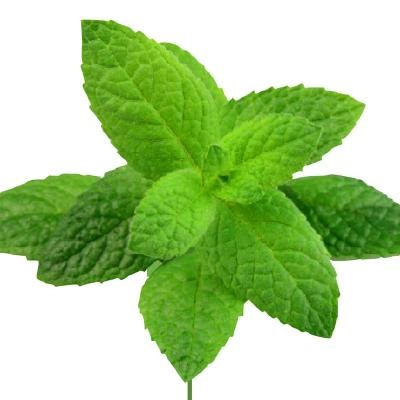
\includegraphics[width=0.18\linewidth]{figures/mi3nts.jpg}\\ 
\vfill

%%%%%%%%%%%%%%%%%%%%%%%%%%%%%%%%%%%%%%%%%%%%%%%%%%%%%%%%%%%%%%%%%%%%
\footnotesize University of Texas at Dallas\\ 
\textit{Department of Physics}\\
\vspace{10pt}
% \textit{Office of Information Technology}\\
% \vspace{10pt}

Multi-Scale Integrated Sensing and Simulation\\ 
\textit{\url{https://mints.utdallas.edu/}}\\
\textit{\url{https://github.com/mi3nts}} \\

\end{flushright}
\end{titlepage}

%%%%%%%%%%%%%%%%%%%%%%
\begin{center}
	\tableofcontents
	\listoftables
	% \listoffigures
\end{center}
\pagebreak

\section{Introduction}
\label{sec:intro}
\pagenumbering{arabic}

The sensing system is an air quality monitor that uses Wi-Fi to transmit measured data. It can also leverage the LoRaWAN communication protocol to send data at a lower rate when Wi-Fi is not available. LoRaWAN’s long-range, low-power design is ideal for remote air quality monitoring. Nonetheless, most VaLo nodes rely on Wi-Fi, which allows for faster data uploads.

\begin{figure}[H]
     \centering
     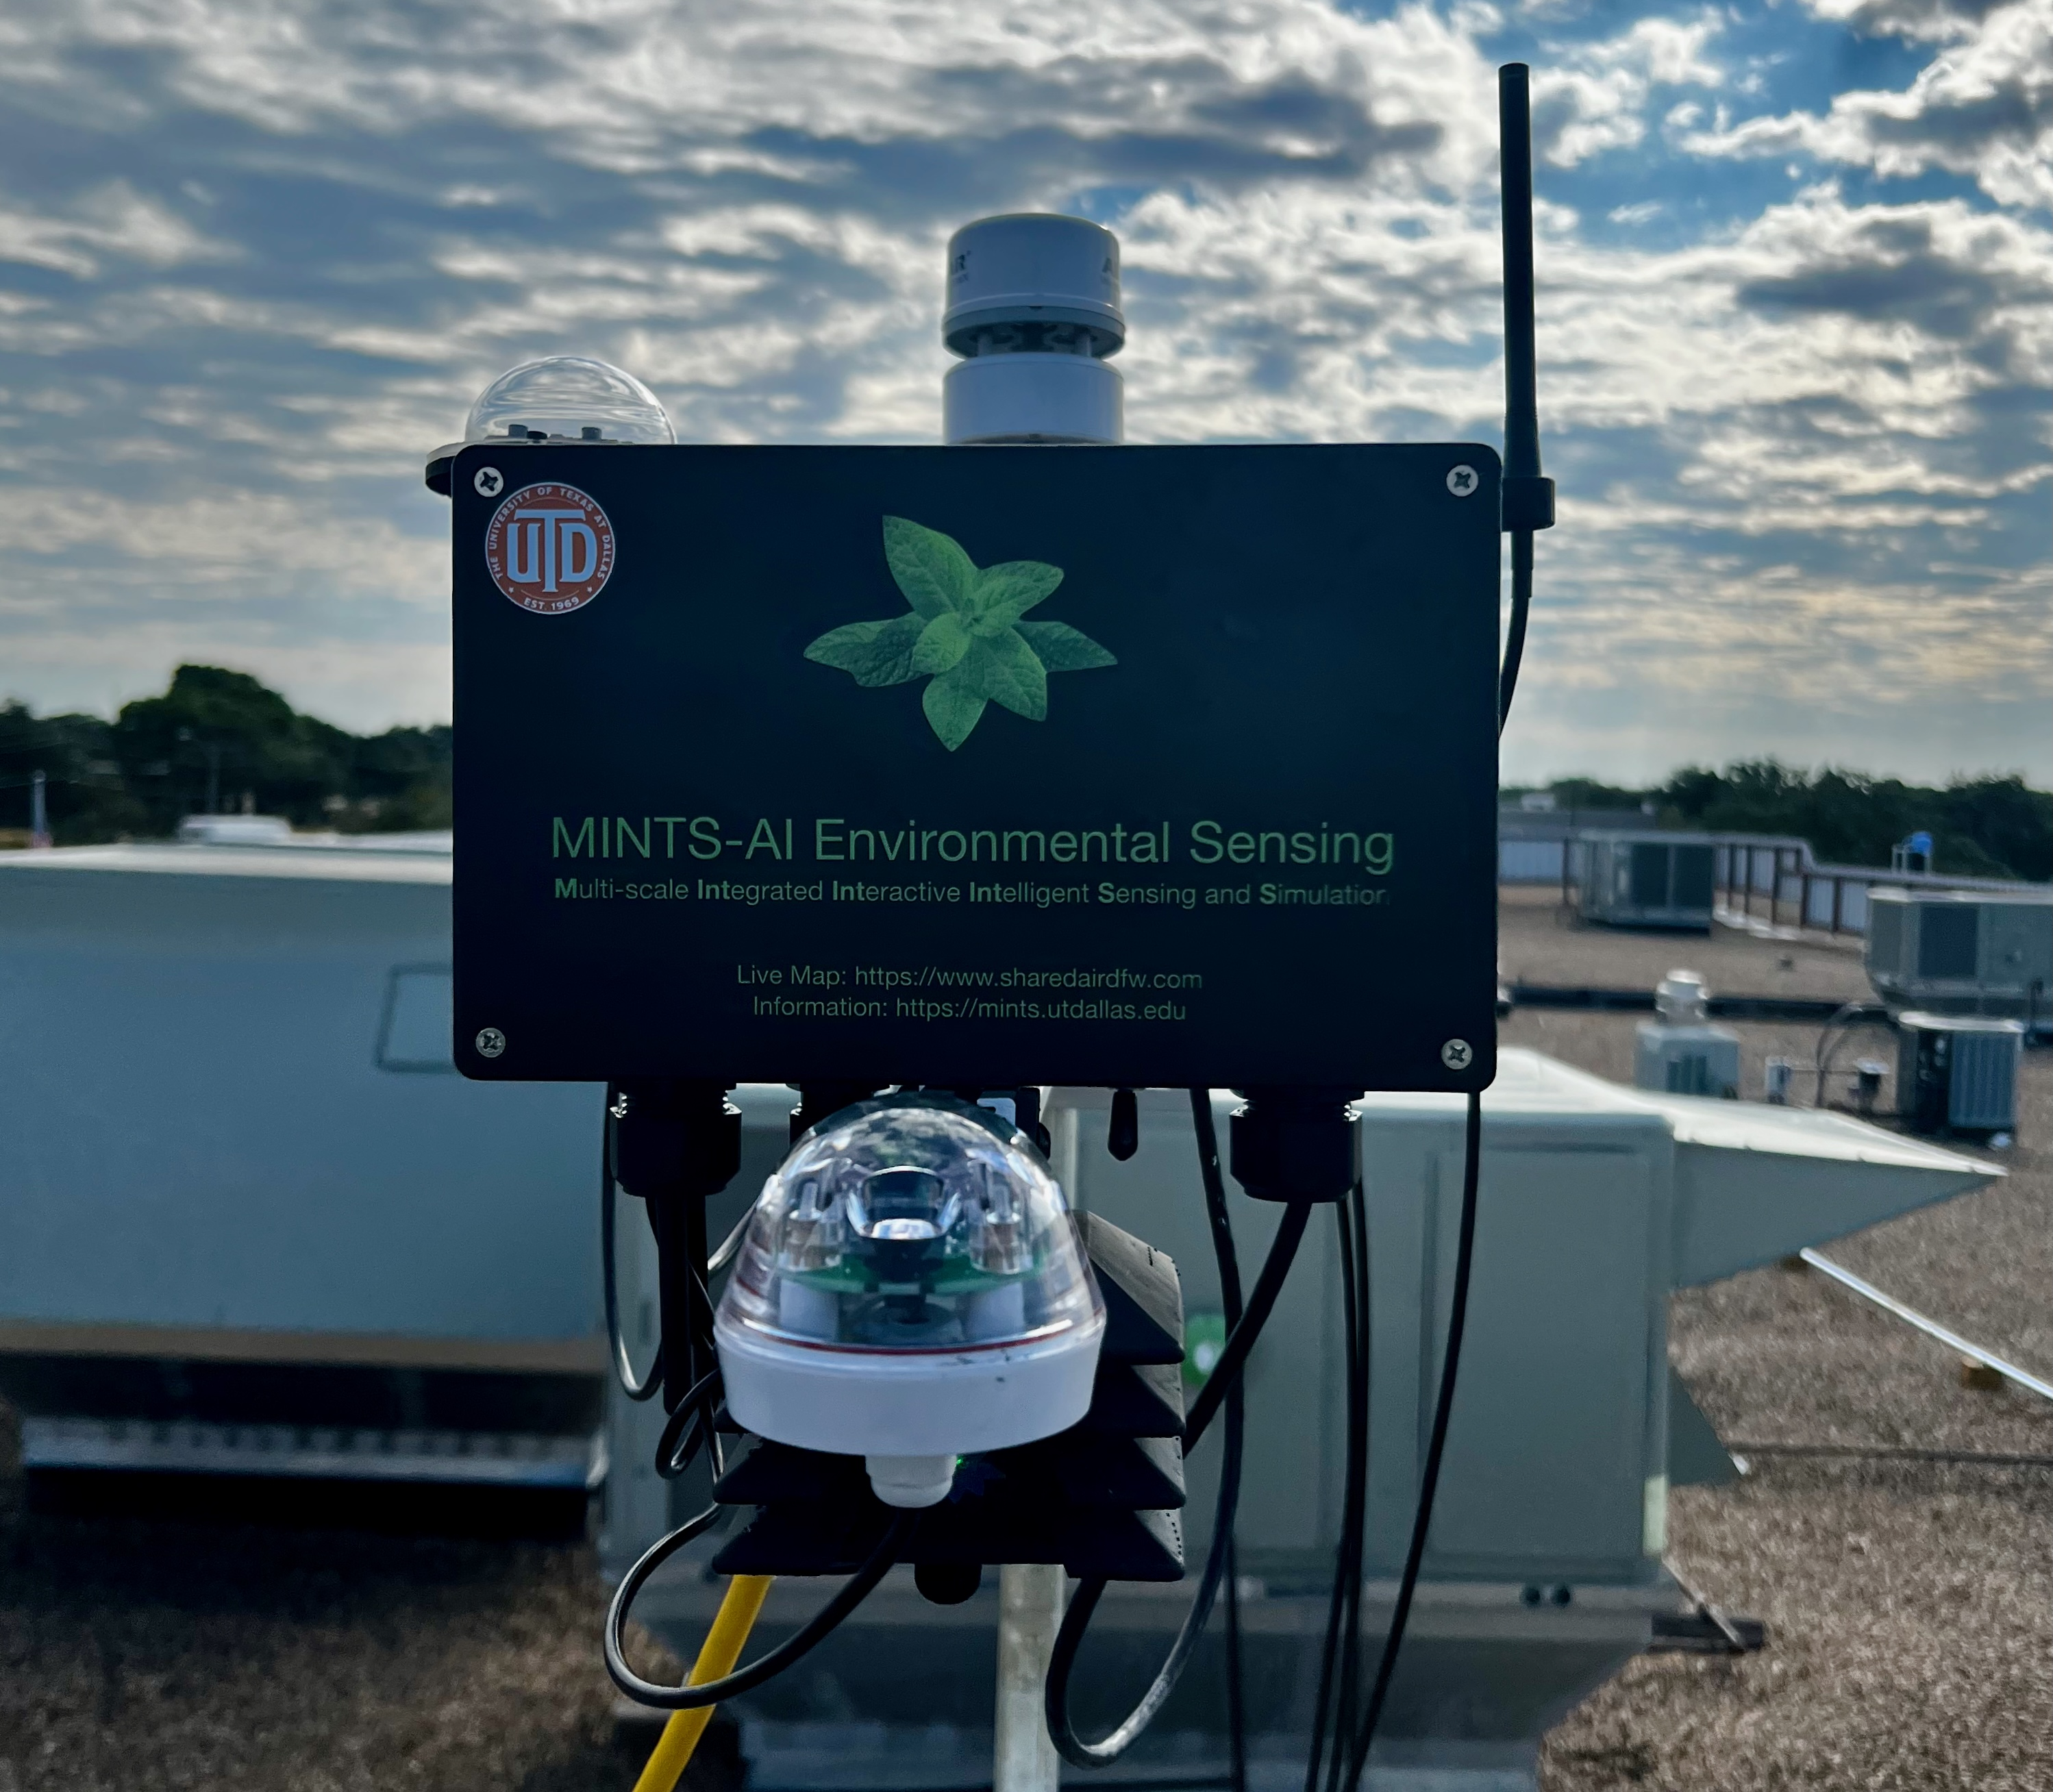
\includegraphics[width=15cm]{figures/valoNode.jpeg}
     \centering
    \caption{VaLo Node Front View}\label{Fig:VaLo Node_1}
\end{figure}

\clearpage

\subsection{Specifications}

\begin{itemize}
    \item Dimensions: 320 * 520 * 400 mm (approximately 12.6 * 20.5 * 16 inches).
    \item Color: Black.
    \item Power: Compatible with Type B socket, providing 120 V, 60 Hz, and 15 amps.
    \item Communication: Supports Wi-Fi (recommended) and LoRaWAN.
    \item Storage: Includes 32 GB of storage.
    \item Intended Usage: Designed for outdoor environments, should be placed away from obvious sources of pollution such as AC vents, ducts, and broilers.
    \item Usage Time: Operates for 2 years with maintenance cycles every 6 months.
\end{itemize}
% \clearpage

\section{Accessories}
The sensing system is devised into modules each tasked with each a unique task. The following list conveys the items comprising each module. 

\begin{itemize}
    \item Compute Module: \href{https://ameridroid.com/products/odroid-c4}{Odroid C4}: 

    The ODROID-C4 4GB is a single-board computer (SBC) that provides a robust and efficient foundation for outdoor sensing units. It is powered by a quad-core ARM Cortex-A55 processor running at 2.016 GHz, delivering the necessary processing power to handle complex data and control operations in sensing applications.
    
    The board includes 4 GB of LPDDR4 RAM, which supports smooth multitasking and efficient data handling. It is equipped with a Mali-G31 MP2 GPU for 4K video playback, useful for high-resolution data visualization.
    
    For connectivity, the ODROID-C4 features USB 3.0 and USB 2.0 ports for interfacing with various peripherals and sensors, as well as HDMI 2.0 for high-quality display output. While Gigabit Ethernet is available, it may not be utilized in the current application. The board offers versatile storage options with support for both eMMC and microSD cards.
    
    The ODROID-C4 4GB runs on Ubuntu in the current application, providing a versatile and robust platform for outdoor sensing units.
    
    \item Power Module: \href{https://www.digikey.com/en/products/detail/cui-inc/VGS-35C-12/13538494}{VGS-35C-12}:
        The VGS-35C-12 is an AC/DC converter designed for efficient and reliable power conversion in various electronic and industrial applications. It converts alternating current (AC) input to direct current (DC) output, providing a stable and consistent power supply for DC-powered devices.
        
        The converter offers a 12V DC output with a power rating of up to 35 watts.
        
    \item Communication Module: 
        The VaLo Nodes are equpped with both a Wi-Fi Radio as well as a LoRaWAN Radio. 
        \begin{itemize}
            \item WiFI Radio - \href{https://ameridroid.com/products/edup-ep-ac1607-wifi-module?_pos=3&_sid=46b124f43&_ss=r}{EDUP EP-AC1607 WiFi Module}: 
            The EDUP EP-AC1607 is a USB Wireless adapter that operates on both 2.4 GHz and 5 GHz bands, compatible with 802.11ac/a/b/g/n standards. It employs the Realtek 8811AU chipset, ensuring reliable connectivity, and boasts a maximum transfer rate of 600Mbps.
            \item LoRaWAN Radio - \href{https://www.seeedstudio.com/LoRa-E5-Wireless-Module-p-4745.html?gad_source=1&gclid=Cj0KCQjwxeyxBhC7ARIsAC7dS3-qwDDoYHPQ9hP4t4SFxPsY7ys7Z9Dv67dw1kYCiV2LP2-xPh-JNXMaAny5EALw_wcB}{LoRaWAN Radio} :
            The STM32WLE5JC, incorporating an ARM Cortex-M4 ultra-low-power MCU and the Long Range SX126X, is engineered to accommodate LoRaWAN frequency plans EU868 and US915. This configuration renders it well-suited for deployment in wireless sensor networks and various IoT contexts demanding stringent battery efficiency, minimal power consumption, and expansive coverage capabilities.
        \end{itemize} 
        
        \item Sensing Module: The sensing module consists of various sensors that gather ambient data on particulate matter, climate, light levels, rain fall, and bird species occupancy. More information on the data payloads from the sensor is given on \ref{sec: sensorPayloads}. 
        Below, you will find the data sheets for each device along with brief descriptions of them.
    
    \begin{itemize}
        \item \href{https://pierasystems.com/wp-content/uploads/2021/12/IPS-Datasheet-V1.1.8.pdf}{IPS7100}: The IPS7100 optical particle counter is capable of detecting particles across a wide range of sizes. Typically, it can measure particles ranging from 0.3 microns to 10 microns in diameter. This range allows the device to provide comprehensive data on various types of particulate matter in the air, including smaller particles such as dust and larger particles such as pollen.
        \item \href{https://www.bosch-sensortec.com/media/boschsensortec/downloads/datasheets/bst-bme280-ds002.pdf}{BME280}:
        The BME280 is a highly integrated environmental sensor designed for measuring atmospheric pressure, humidity, and temperature. It is known for its high accuracy and low power consumption.
        
        \item \href{https://rainsensors.com/products/rg-15/}{RG15}: The RG15 is a versatile weather sensor that measures rain. It features a rugged, reliable, maintenance-free and accurate detection system that uses an optical technology to measure precipitation rate and accumulation.
        
        \item \href{https://sensirion.com/media/documents/4EAF6AF8/61652C3C/Sensirion_CO2_Sensors_SCD30_Datasheet.pdf}{SCD30} The SCD30 is a sensor module that accurately measures carbon dioxide (CO$_2$), relative humidity, and temperature. Utilizing non-dispersive infrared (NDIR) technology, the SCD30 provides precise CO$_2$ readings across a range from 400 to 10,000 ppm. 
        \item \href{https://cdn.sparkfun.com/assets/c/2/9/0/a/AS7265x_Datasheet.pdf?_gl=1*nuz15w*_ga*MzMxOTM2OTQwLjE2OTAyMzE1NzI.*_ga_T369JS7J9N*MTY5MDIzMTU3MS4xLjAuMTY5MDIzMTU3MS42MC4wLjA.}{AS7265x}: The AS7265X is a triad of multispectral sensors that measures light across 18 channels, spanning the visible and near-infrared (NIR) spectrum. These sensors cover wavelengths from 410 nm (violet) to 940 nm (NIR) in 20 nm increments. The AS7265X consists of three devices: AS72651, AS72652, and AS72653, each responsible for different parts of the spectrum
        \item \href{https://cdn-learn.adafruit.com/downloads/pdf/adafruit-mini-gps-pa1010d-module.pdf}{PA101D}: 
        The PA101D is a GPS (Global Positioning System)  module designed for accurate positioning and navigation. It offers high-sensitivity signal reception and quick acquisition times, supporting multiple satellite systems such as GPS and GLONASS for enhanced accuracy. The module features digital communication interfaces like UART for easy integration and low power consumption, making it suitable for portable devices and IoT applications such as the current one.
        \end{itemize}        
\end{itemize}

%  Add Later 
% The following table gives some valuable information on each accessory. 

% \begin{longtable}{|p{2cm}|p{4.5cm}|}
%   \caption{VaLo Node Components} \label{t:dataFormatTbl1} \\
%   \hline
%   \centering Accessory &  \\
%   \hline \hline

%   \hline
% \end{longtable}

% \begin{longtable}{|p{2cm}|p{4.5cm}|}
%   \caption{VaLo Node Components} \label{t:dataFormatTbl1} \\
%   \hline
%   \centering Sensor Nodes & VaLo  Node \\
%   \hline \hline
%   Sketches & 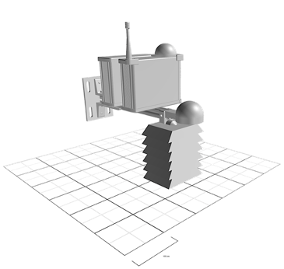
\includegraphics[width=3cm]{figures/PoLo_2.png} \\
%   \hline
%   SBC & \href{https://ameridroid.com/products/odroid-c4}{Odroid C4} \\
%   \hline
%   Attached sensors & 
%         \begin{itemize}
%           \item \href{https://pierasystems.com/wp-content/uploads/2021/12/IPS-Datasheet-V1.1.8.pdf}{IPS7100}
%         \item \href{https://www.bosch-sensortec.com/media/boschsensortec/downloads/datasheets/bst-bme280-ds002.pdf}{BME280 (Version 2)}
%         \item \href{https://www.bosch-sensortec.com/media/boschsensortec/downloads/datasheets/bst-bme688-ds000.pdf}{BME688}
%         \item \href{https://rainsensors.com/products/rg-15/}{RG15}
%         \item \href{https://sensirion.com/media/documents/4EAF6AF8/61652C3C/Sensirion_CO2_Sensors_SCD30_Datasheet.pdf}{SCD30}
%         \item \href{https://cdn.sparkfun.com/assets/c/2/9/0/a/AS7265x_Datasheet.pdf?_gl=1*nuz15w*_ga*MzMxOTM2OTQwLjE2OTAyMzE1NzI.*_ga_T369JS7J9N*MTY5MDIzMTU3MS4xLjAuMTY5MDIzMTU3MS42MC4wLjA.}{AS7265x}
%         \item \href{https://cdn-learn.adafruit.com/downloads/pdf/adafruit-mini-gps-pa1010d-module.pdf}{GPGGAPL}
%         \item \href{https://cdn-learn.adafruit.com/downloads/pdf/adafruit-mini-gps-pa1010d-module.pdf}{GPRMCPL}
%         \end{itemize}
%   \hline
% \end{longtable}



\section{Installation of VA's Powered LoRa WAN (VaLo) Nodes and Gateway}
\subsection{Steps for Installing VaLo Nodes}
Please follow the steps given below to install each of the VaLo Nodes:
\begin{itemize}
\item The picture below shows how the VaLo Node needs to be positioned on the wall or the mounting surface. First, the antenna should point upward, towards the sky. Then, ensure that the Mints logo is upright and facing you as given in the picture.
 \begin{figure}[H]
     \centering
     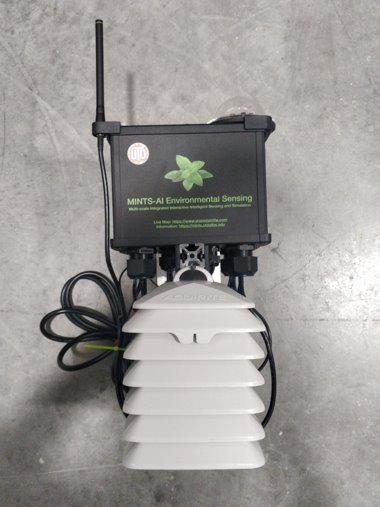
\includegraphics[width=12cm,height=12cm,]{figures/VaLo_1.png}
     \centering
    \caption{VaLo Node Front View}\label{Fig:VaLo Node_1}
\end{figure}
\item The picture below shows the side view of the node once it has been positioned correctly.
 \begin{figure}[H]
     \centering
     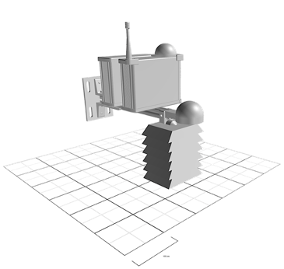
\includegraphics[width=12cm,height=12cm,]{figures/VaLo_2.png}
     \centering
    \caption{VaLo Node Side View}\label{Fig:VaLo Node_2}
\end{figure}
\item  The wall/pole base plate specs can be found here: \url{https://www.mcmaster.com/3136N138/}
\item The base plate can either be mounted on a pole, a wall, or a non-penetrative roof-mount base.
\item The holes on the base  plate are roughly 2.36 - 3.18 inches apart, so a U-Bolt of Center -to-Center	2 11/16"" inches should be good to use. The link to the product is given here:
\url{https://www.mcmaster.com/3042T78/}
\item Alternatively, you can use  screws/nuts or even nails depending on where you want it to be mounted.
\item Once the base plate has been mounted, the node can be plugged into any standard 120V, 60Hz socket.
\item Once it's plugged in, switch ON the VaLo node to power it up.
\end{itemize}
\subsection{Steps for Installing Va's Powered Lora WAN Gateway Module}
\begin{itemize}
    \item The VaLo Gateway Module can be installed in a similar fashion as the VaLo Node. Please make sure the MINTS Logo is up right, facing you, and all the 4 inlets are facing downwards.
    \begin{figure}[H]
         \centering
        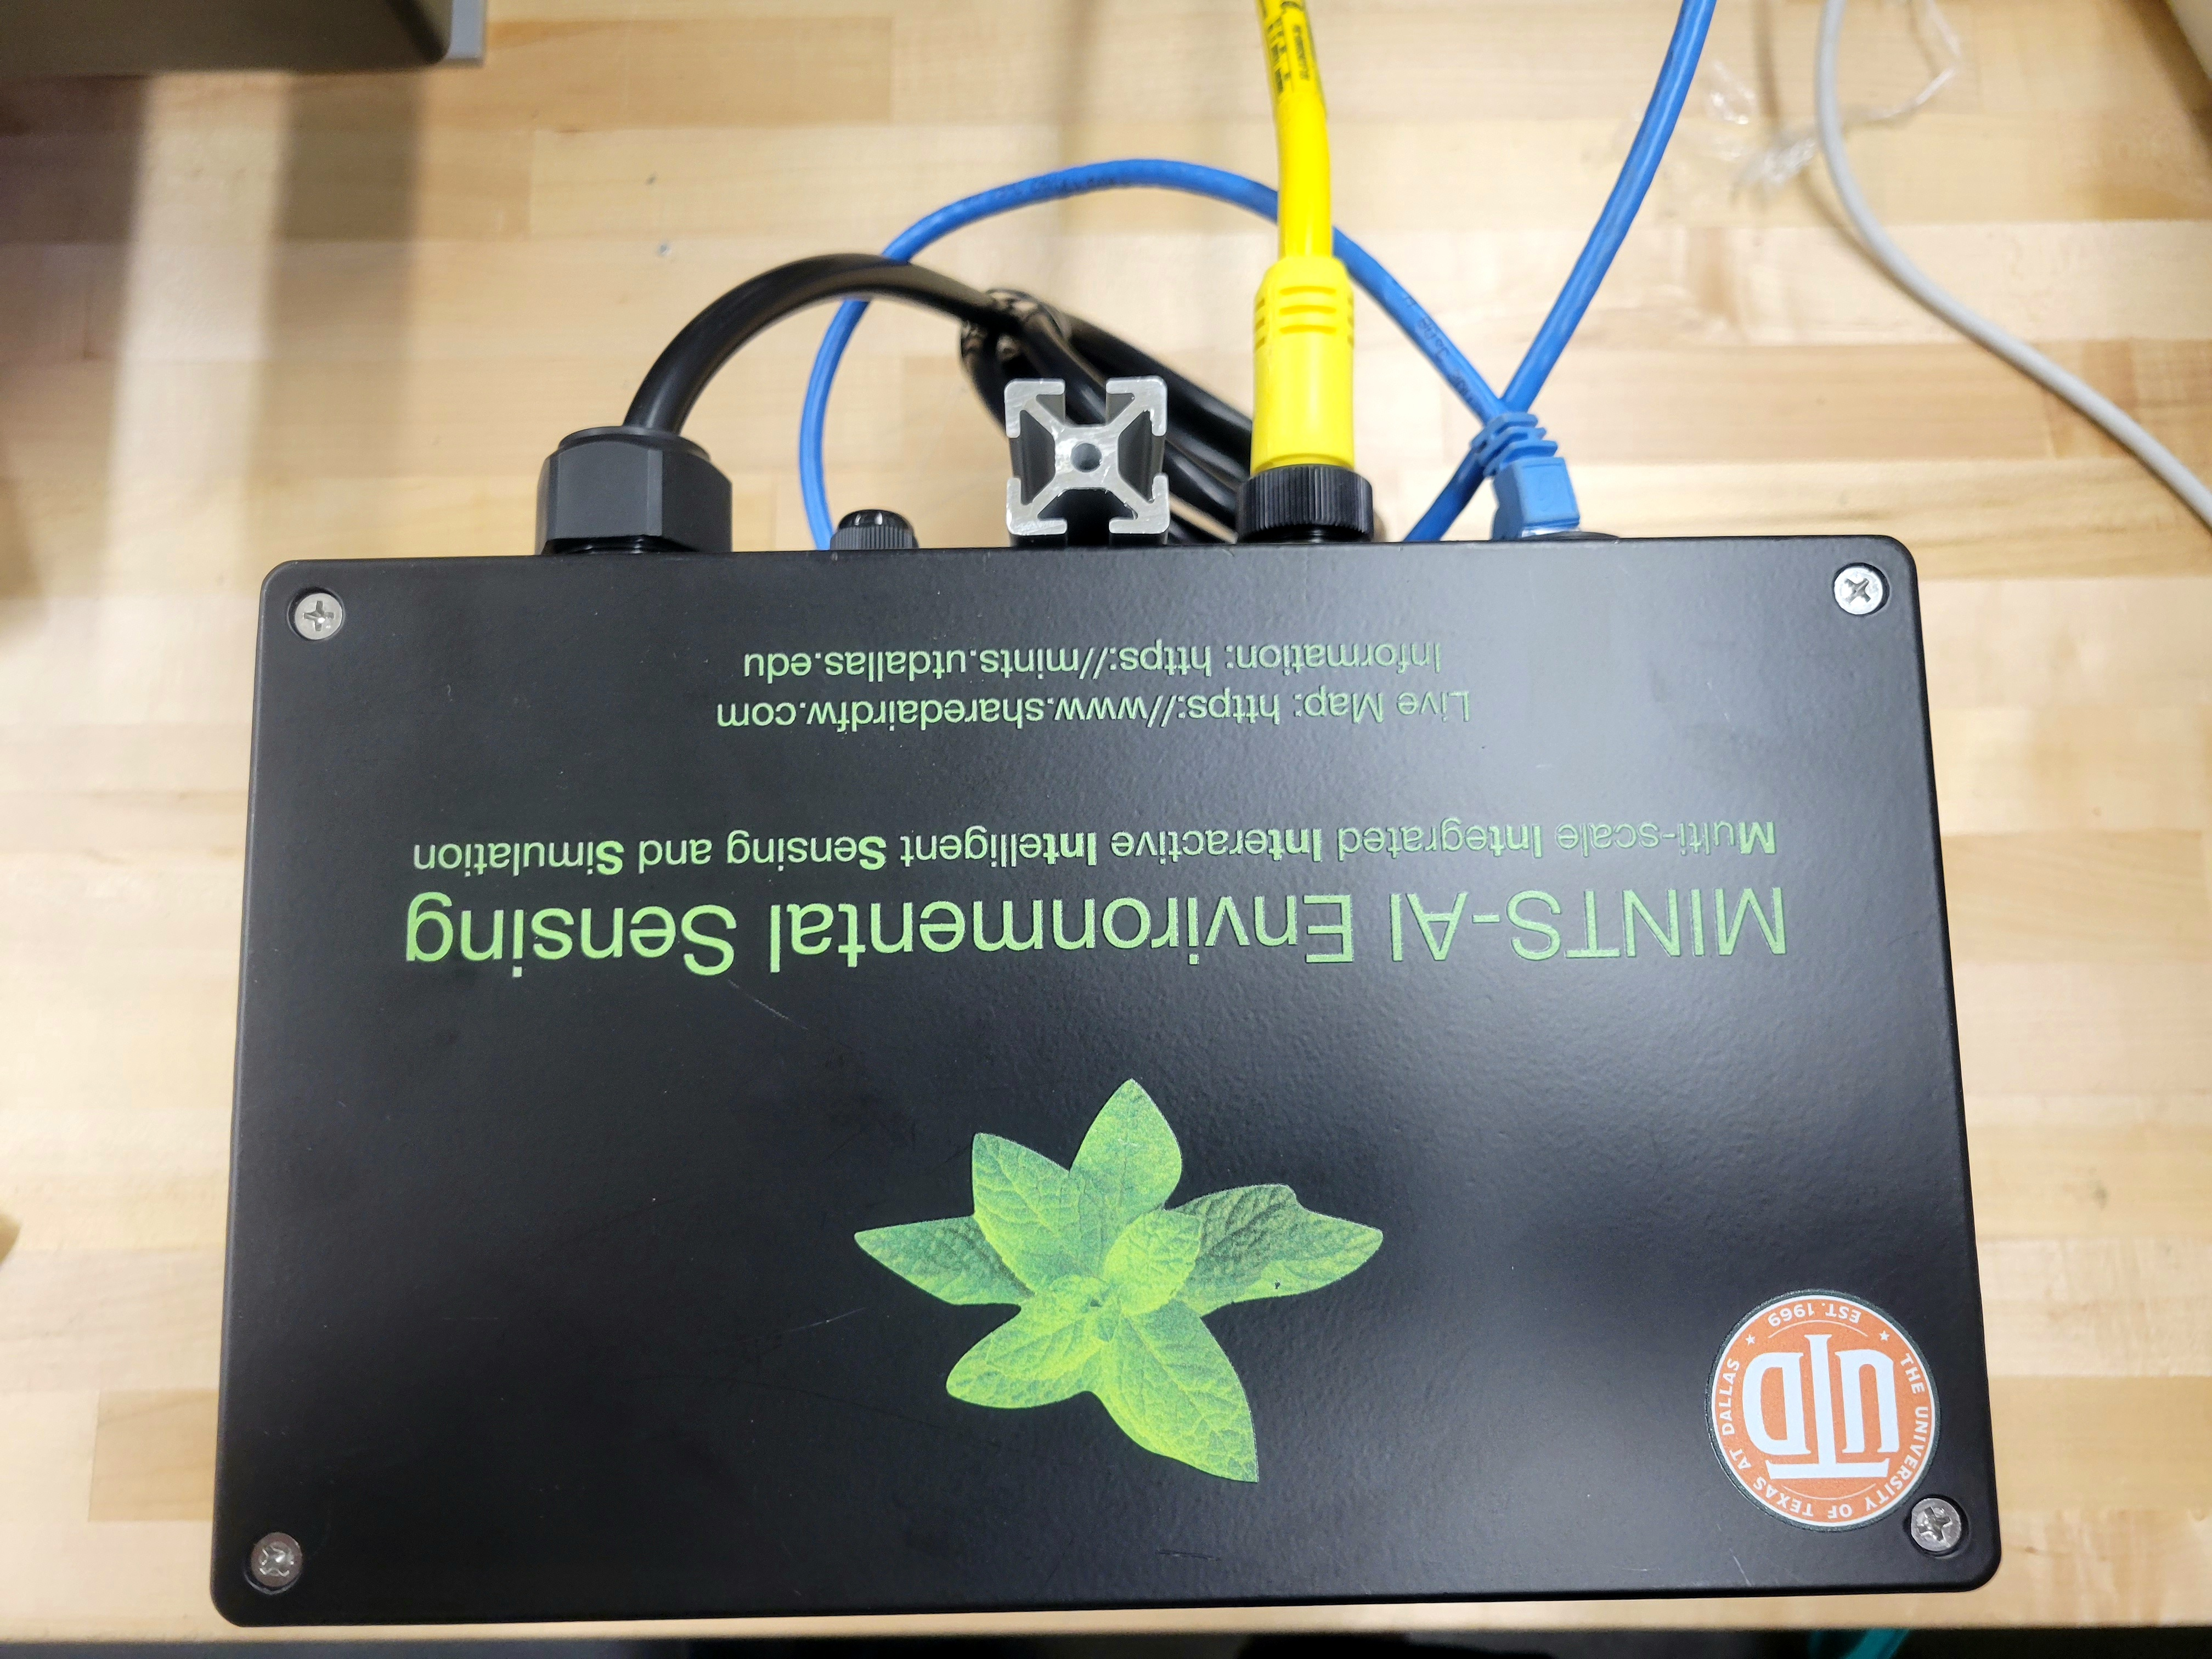
\includegraphics[width=12cm,height=12cm,angle=180]{figures/gateway.jpg}
         \centering
        \caption{Gateway Node Position}\label{Fig:Gateway Node Position}
    \end{figure}
    \item Once it's positioned correctly, it will look as shown in the figure given below:
     \begin{figure}[H]
         \centering
         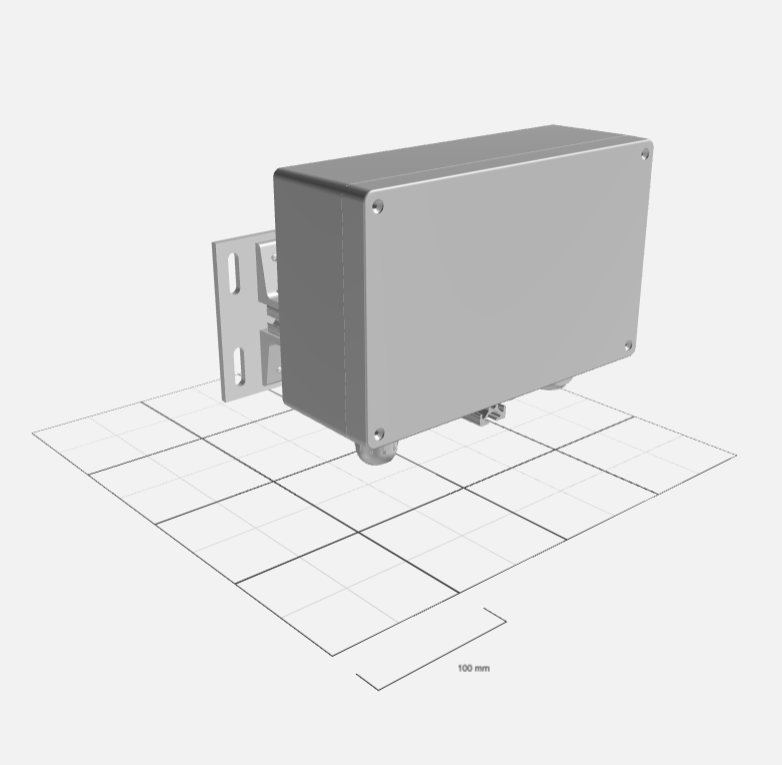
\includegraphics[width=12cm,height=12cm,]{figures/gateway_1.png}
         \centering
        \caption{Gateway Node}\label{Fig:Gateway Node}
    \end{figure}
    \item The gateway module has the same base plate as the VaLo node and can be mounted in a similar manner. The gateway module has four inlets, as displayed below: 
    \begin{figure}[H]
         \centering
         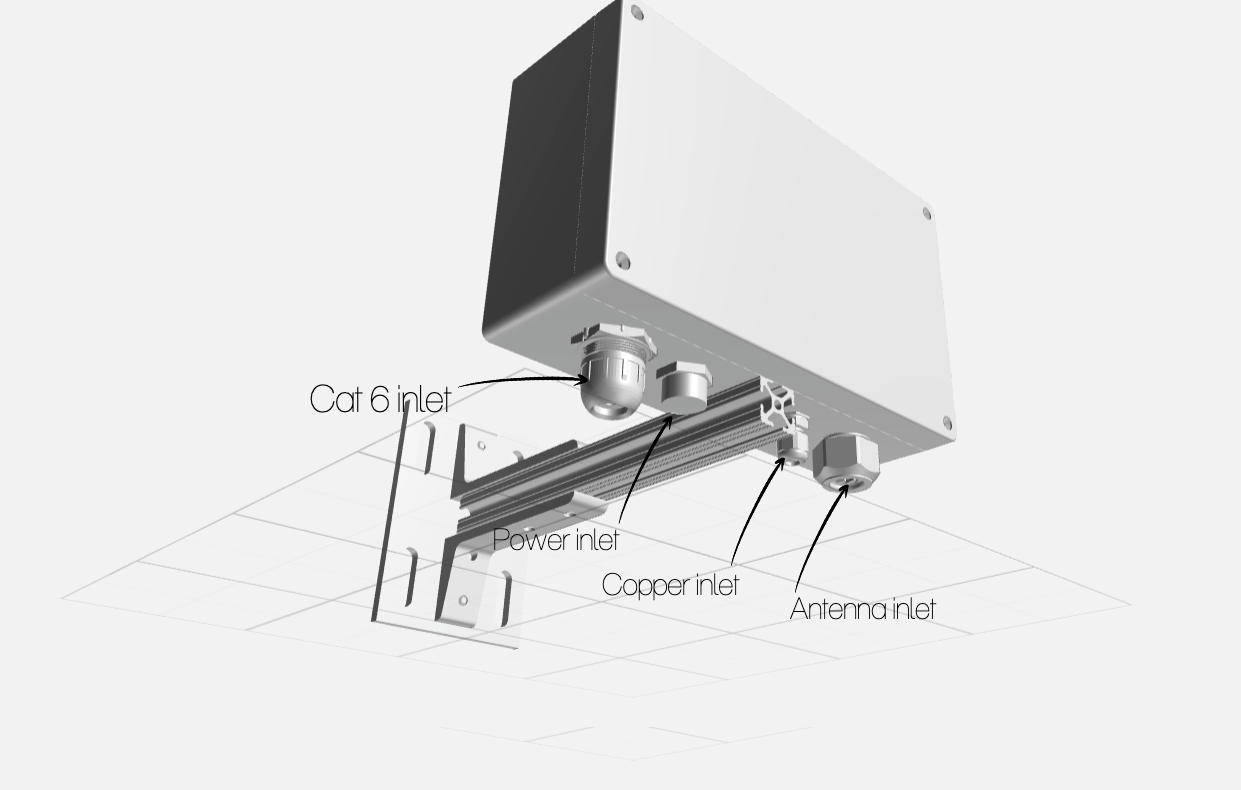
\includegraphics[width=12cm,height=8cm,]{figures/gateway_2.png}
         \centering
        \caption{Gateway Node Inlets}\label{Fig:Gateway Node Inlets}
    \end{figure}
\item You can follow the instructions given below to provide the connections to each of the inlets:
    \begin{enumerate}
        \item \textit{Cat 6 Inlet:} A black Ethernet cable is included for connection. It can be inserted into a Cat 6 inlet.
        \item  \textit{Power Inlet:} A yellow power cable is provided. The system can be plugged into any standard 120 V, 60 Hz socket.
        \item  \textit{Copper Conductor Wire Inlet (cable not included):} The gateway module incorporates a built-in lightning arrester. One end of the copper wire should be connected to the lightning arrester, while the other end must be properly grounded. Grounding is essential for the lightning arrester's effective operation.
                \begin{figure}[H]
             \centering
             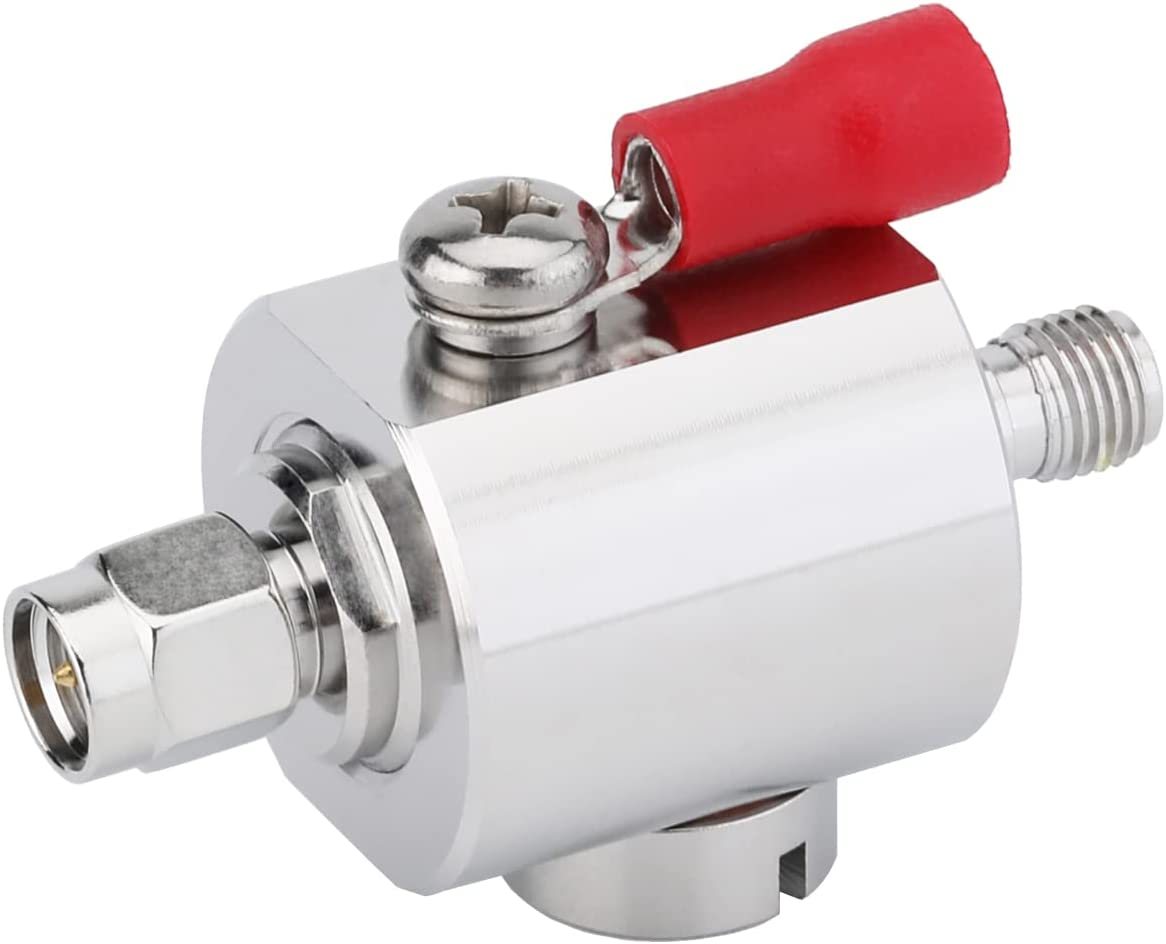
\includegraphics[width=6cm,height=4cm,]{figures/lightning_protection.jpg}
             \centering
            \caption{SMA Lightning Arrester Protect}\label{Fig:SMA Lightning Arrester Protect}
        \end{figure}
        
        \item \textit{Antenna Inlet:} The gateway module requires connection to a 915 MHz antenna. 
        
        \begin{figure}[H]
             \centering
             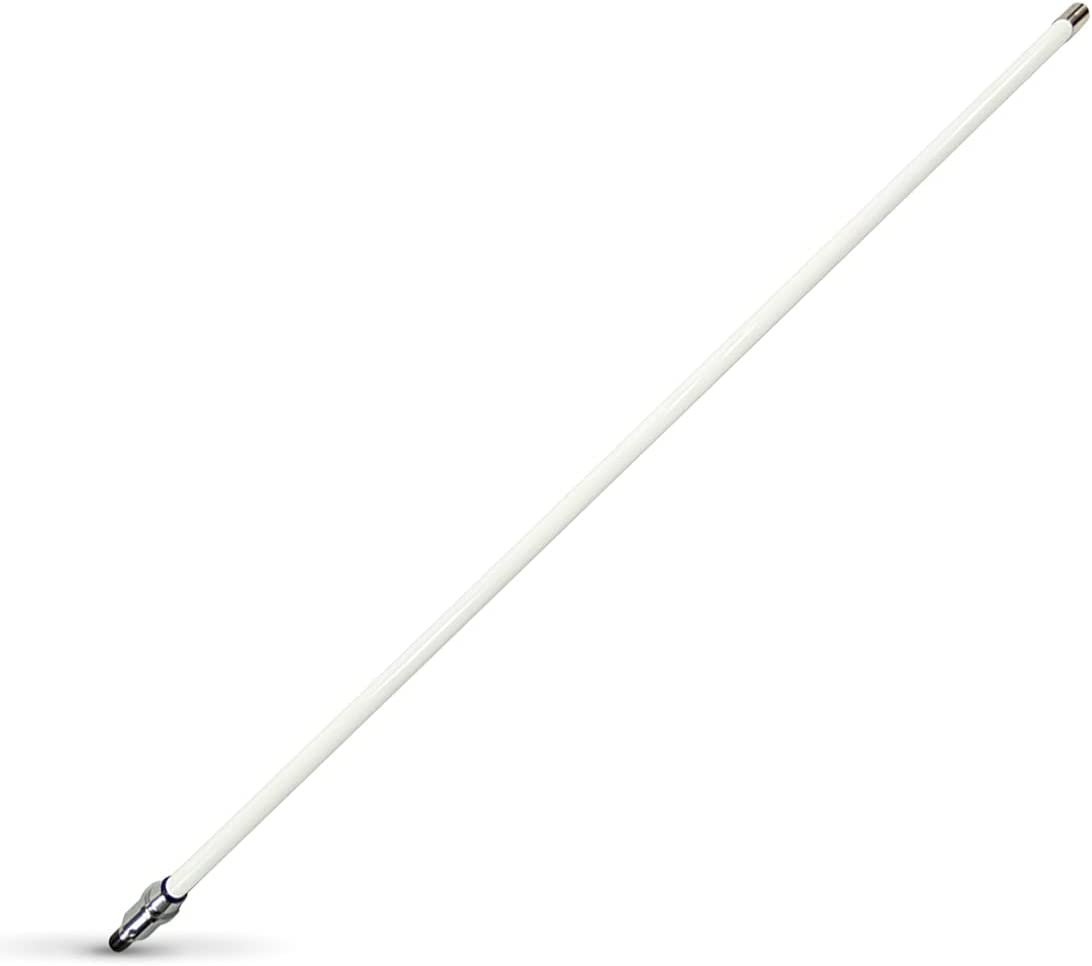
\includegraphics[width=12cm,height=6cm,]{figures/antenna.png}
             \centering
            \caption{915 MHz Antenna}\label{Fig:Antenna}
        \end{figure}
        
        The 915 MHz antenna should be mounted in a suitable location, away from obstacles such as walls, to optimize communication with the VaLo nodes. The antenna comes with a cylindrical metal mounting point, which can be mounted separately. \textbf{(Note: The antenna cable is passed through the cylindrical frame and connected to the antenna base. The antenna connection is secured with the help of the screw ). Please make sure to use liquid electrical tape to seal the gap between the screw and the antenna to make it weather proof.}
        \begin{figure}[H]
             \centering
             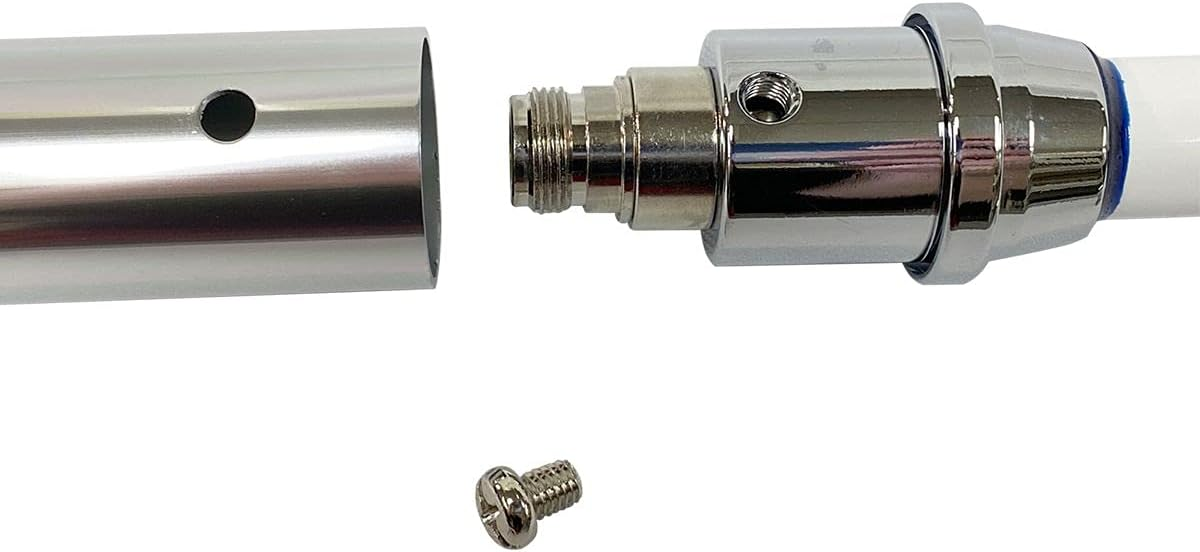
\includegraphics[width=12cm,height=8cm,]{figures/antenna_mount.png}
             \centering
            \caption{Antenna's Cylindrical Mounting Point}\label{Fig:Cylindrical Mounting Point}
        \end{figure}
        
        It's recommended to inspect these mounts before finalizing their placement. The circular mount can be secured using u-bolts, pipe hangers, or clamps, depending on the location. The diameter of the cylindrical frame is 1.26".A Ubolt with Center -to-Center width 1 3/4" will be sufficient. The link to that is given below: \url{https://www.mcmaster.com/3042T69/}
 \end{enumerate}

\end{itemize}





\textit{Important Note: The VaLo Node should be serviced once in every 6 months}


\section{Sensor Payloads}\label{sec:sensorPayloads}
 Data from each VaLo  Node is initially saved as \emph{csv} files. There is a Single board computer (OdroidC4) that records the data from each of the sensor. The SBC has an unique node id and a group of sensors connected to it. A \emph{csv} file is provided for each sensor within a VaLo node per day and is collected under the  node id. In order to maintain a record of the most recent data read, a unique json file is updated for each individual sensor. Upon connection to the internet both the \emph{csv} and \emph{json} files are transferred via \emph{rsync} \cite{tridgell1996rsync}. Upon transmission the data to the graphical dashboards are updated using an \emph{mqtt} \cite{Light2017} pipeline. For each day, each sensor will have a single csv file saved inside the respective node, with the following folder structure @ \emph{\textbackslash mfs\textbackslash io\textbackslash groups\textbackslash lary \textbackslash mintsData}.

 
  \begin{minted}{java}
    ├── mintsData
        └── rawMqtt
            └── 2cf7f1203230480a
                └── 2023
                    └── 08
                        └── 04
                            ├── MINTS_2cf7f1203230480a_AS7265X_2023_08_04.csv
                            ├── MINTS_2cf7f1203230480a_BME688CNR_2023_08_04.csv
                            ├── MINTS_2cf7f1203230480a_GPGGAPL_2023_08_04.csv
                            ├── MINTS_2cf7f1203230480a_GPRMCPL_2023_08_04.csv
                            ├── MINTS_2cf7f1203230480a_IPS7100CNR_2023_08_04.csv
                            ├── MINTS_2cf7f1203230480a_SCD30_2023_08_04.csv
    \end{minted}  
    

In this example, the sensor ID happens to be \emph{2cf7f1203230480a} which is the unique ID corresponding to the OdroidC4.
\clearpage

\subsection{Equipped Sensing Modules}
\subsubsection{Particle Counters}
\paragraph{IPS7100}
\label{sec:ips7100DataFormat}
{
\begin{minted}{java}
dateTime                     pc0_1    pc0_3    pc0_5    ......  pm10_0
2023-08-04 00:00:14.263430   64474    18205    11661    ......  5.74317020
2023-08-04 00:00:31.311544   62047    17368    11109    ......  5.57649617
2023-08-04 00:00:39.338181   59468    16571    10640    ......  5.40531891
2023-08-04 00:00:57.375111   56790    15791    10198    ......  5.23171629
2023-08-04 00:01:14.282239   54282    15017    9777     ......  5.06503846
2023-08-04 00:01:30.313624   51981    14281    9377     ......  4.90459504
2023-08-04 00:01:38.828155   49793    13580    9015     ......  4.76209408
\end{minted} }
The data format of the \textbf{IPS7100} \emph{csv} is described on table \ref{t:dataFormatips7100}.   
    \begin{table}[H]
	\caption{Data Format used on the \textbf{IPS7100} data \emph{csv}}
	 \label{t:dataFormatips7100}
	\small
	\begin{tabular}{||p{2cm}| p{2cm}|p{2cm}|p{1.5cm}|p{1.5cm}|p{2cm}|p{2cm}||}
	
		\hline
		\hline
		Parameter & Column Name & Format & Unit & Errors & Example & Comments \\ \hline
    	\hline
	    UTC Time & dateTime & yyyy-MM-dd hh:mm:ss & & &\tiny{2023-08-04 00:00:02.263430}   &  \\
        \hline
		Particles Counts & pc0\_1 to pc10\_0 & Integer & $\#/Liter$ & Particle Counts per $liter$ for particle diameters 0.1, 0.3, 0.5, 1.0, 2.5, 5, 10 $\mu$m & 3272 &\\
		    \hline
		Particulate mass \hbox{fractions} & pm0\_1 to pm10\_0 & Float & $\mu$g/m$^{3}$ & Particle mass fractions for particle diameters 0.1, 0.3, 0.5, 1.0, 2.5, 5, 10 $\mu$m & 2.56 &\\
	    \hline
		\hline
	\end{tabular}
\end{table}
\clearpage

\subsubsection{Climate Sensors}

\paragraph{BME280  (Version 2)}
    \label{sec:bme280DataFormat}
        {\begin{minted}{java}
dateTime                     temperature   pressure    ......... altitude
2023-08-04 00:00:06.268466   40.53         986.33      ......... 149.66
2023-08-04 00:00:16.296297   40.58         986.36      ......... 149.49
2023-08-04 00:00:26.309238   40.44         986.25      ......... 149.91
2023-08-04 00:00:36.337023   40.08         986.28      ......... 149.83
2023-08-04 00:00:46.350128   39.87         986.28      ......... 149.75
2023-08-04 00:00:56.362813   39.81         986.28      ......... 149.75
2023-08-04 00:01:06.390603   39.64         986.28      ......... 149.75
\end{minted} }
The data format of the \textbf{BME280} \emph{csv} is described on table \ref{t:dataFormatbme280}.
        \begin{table}[H]
    	\caption{Data format used on \textbf{BME280} data \emph{csv}}
    	 \label{t:dataFormatbme280}
    	\small
    	\begin{tabular}{||p{2cm}| p{2cm}|p{2cm}|p{1.5cm}|p{1.5cm}|p{2cm}|p{2cm}||}
    		\hline
    		\hline
    		Parameter & Column Name & Format & Unit & Errors & Example & Comments \\ 
            \hline
            \hline
    	    UTC Time & dateTime & yyyy-MM-dd hh:mm:ss & & & \tiny 2023-01-04 00:00:06.268466 &  \\
    	    \hline
    		Temperature & temperature  & Float & 
               $ ^{\circ} C$  & &40.81 &  \\
               	\hline
    		Pressure & pressure  & Float & 
               hPa  & & 986.33 &  \\
               	\hline
    		Humidity & humidity  & Float & 
               $ \% $  & & 29.00 & \\
                \hline

            Dew Point & dewPoint  & Float & 
               $ ^{\circ} C$  & & 18.75 & \\
                \hline
    		Altitude & altitude  & Float & 
               meters  & & 149.66 & \\
               	\hline
    		\hline
    	\end{tabular}
    \end{table}
    \clearpage
    
\paragraph{BME688}
    \label{sec:bme688DataFormat}
        {\begin{minted}{java}
dateTime                     temperature          ...... co2Eq
2023-08-04 00:00:10.173226   40.630001068115234   ...... 642.989990234375
2023-08-04 00:01:50.746008   40.83000183105469    ...... 646.859985351562
2023-08-04 00:03:31.323085   40.599998474121094   ...... 632.320007324218
2023-08-04 00:05:11.821272   40.279998779296875   ...... 633.280029296875
2023-08-04 00:06:52.403963   40.33000183105469    ...... 625.710021972656
2023-08-04 00:08:32.982740   40.209999084472656   ...... 632.849975585937
2023-08-04 00:10:13.428428   40.439998626708984   ...... 641.239990234375
\end{minted} }
The data format of the \textbf{BME688} \emph{csv} is described on table \ref{t:dataFormatbme688}.
        \begin{table}[H]
    	\caption{Data format used on \textbf{BME688} data \emph{csv}}
    	 \label{t:dataFormatbme688}
    	\small
    	\begin{tabular}{||p{2cm}| p{2cm}|p{2cm}|p{1.5cm}|p{1.5cm}|p{2cm}|p{2cm}||}
    		\hline
    		\hline
    		Parameter & Column Name & Format & Unit & Errors & Example & Comments \\ 
            \hline
            \hline
    	    UTC Time & dateTime & yyyy-MM-dd hh:mm:ss & & & \tiny 2023-08-04 00:00:10.173226 &  \\
    	    \hline
    		Temperature & temperature  & Float & 
               $ ^{\circ} C$  & \hbox{$\pm$0.5 $^{\circ}$C} for \hbox{(0 - 65 $^{\circ}$C )}& \tiny 40.630001068115234 &  \\
               	\hline
    		Humidity & humidity  & Float & 
               $ \% $  & \hbox{$\pm$3$\%$ r.H.} & \tiny 25.059999465942383 & \\
                \hline
                Pressure & pressure  & Float & 
               Pa  &    \tiny $\pm$1.3 Pa/K which is equivalent to $\pm$10.9 cm change at \hbox{1 $^{\circ}$C} \hbox{temperature} change & \tiny  985.5499877929688  &  \\
               	\hline
    		Air Qulaity Index & vocAqi    & Float & 
                 & &  \tiny 64.45999908447266   & \\
                \hline
    		Volatile Organic Compounds in Breath & bvocEq   & Float & 
               ppm  & & \tiny 0.8600000143051147 & \\
                \hline 
    		\hbox{Gas} \hbox{Estimation} & gasEst   & Float & 
               \%  & & \tiny 0.0  & \\
                \hline
    		CO$_{2}$ & co2Eq  & Float & 
               ppm  & & \tiny 642.989990234375 & \\
               	\hline
    		\hline
    	\end{tabular}
    \end{table}
\clearpage

\paragraph{RG15}
    \label{sec:rg15DataFormat}
        {\begin{minted}{java}
dateTime                     accumulation ...............  rainPerInterval
2023-08-04 00:01:06.200348   0.00         ...............  0.00
2023-08-04 00:02:56.201240   0.00         ...............  0.00    
2023-08-04 00:04:37.204291   0.00         ...............  0.00   
2023-08-04 00:06:18.207039   0.00         ...............  0.00   
2023-08-04 00:08:00.209195   0.00         ...............  0.00   
2023-08-04 00:09:41.212983   0.00         ...............  0.00   
\end{minted} }
         The data format of the \textbf{RG15} \emph{csv} is described on table \ref{t:dataFormatrg15}.
        
        
        \begin{table}[H]
    	\caption{Data format used on \textbf{RG15} data \emph{csv}}
    	 \label{t:dataFormatrg15}
    	\small
    	\begin{tabular}{||p{2cm}| p{2cm}|p{2cm}|p{1.5cm}|p{1.5cm}|p{2cm}|p{2cm}||}
    		\hline
    		\hline
    		Parameter & Column Name & Format & Unit & Errors & Example & Comments \\ 
            \hline
            \hline
    	    UTC Time & dateTime & yyyy-MM-dd hh:mm:ss & & & \tiny 2023-07-26 00:00:07.200348 &  \\
    	    \hline
    		Accumulation & accumulation  & Float & & & 0.00 &  \\
               	\hline
    		Event \hbox{Accumulation} & event \hbox{Accumulation}  & Float & 
                & & 0.00 &  \\
                	\hline
    		Total \hbox{Accumulation} & total \hbox{Accumulation}  & Float & 
                & & 0.00 &   \\
                \hline
    		Rain Per  \hbox{Interval} & rainPer \hbox{Interval}  & Float & 
               & & 0.00 &   \\
               	\hline
    		\hline
    	\end{tabular}
    \end{table}
\clearpage

\subsubsection{Gas Sensors}
\paragraph{SCD30}
\label{sec:scd30DataFormat}
{\begin{minted}{java}
dateTime                     c02   temperature   humidity
2023-08-04 00:00:08.763232   405   19.44         27.58
2023-08-04 00:00:18.775858   406   19.44         27.53
2023-08-04 00:00:28.803976   405   19.42         27.62
2023-08-04 00:00:38.816727   405   19.44         27.64
2023-08-04 00:00:48.829733   405   19.44         27.59
2023-08-04 00:00:58.857351   406   19.44         27.62

\end{minted} }
The data format of the \textbf{SCD30} \emph{csv} is described on table \ref{t:dataFormatscd30}.
    
        
        \begin{table}[H]
    	\caption{Data format used on \textbf{SCD30} data \emph{csv}}
    	 \label{t:dataFormatscd30}
    	\small
    	\begin{tabular}{||p{2cm}| p{2cm}|p{2cm}|p{1.5cm}|p{1.5cm}|p{2cm}|p{2cm}||}
    		\hline
    		\hline
    		Parameter & Column Name & Format & Unit & Errors & Example & Comments \\ 
            \hline
            \hline
    	    UTC Time & dateTime & yyyy-MM-dd hh:mm:ss & & & \tiny 2023-01-04 00:00:04.568350 &  \\
            \hline
    		CO$_{2}$ & co2  & Integer & 
               ppm  & & 405 &   \\
    	    \hline
    		Temperature & temperature  & Float & 
               $ ^{\circ} C$  & & 19.44 &  \\
               	\hline
    		Humidity & humidity  & Float & 
               $ \% $  & & 27.58 &   \\

               	\hline
    		\hline
    	\end{tabular}
    \end{table}


\subsubsection{Light Sensors}
\paragraph{AS7265X}
\label{sec:as7265DataFormat}
{\begin{minted}{java}
dateTime                     channelA410nm        .......... channelL940nm
2023-08-04 00:01:01.324491   96.16065216064453    .......... 10.99194336
2023-08-04 00:02:41.871354   92.7263412475586     .......... 10.99194336
2023-08-04 00:04:22.378722   90.1506118774414     .......... 10.99194336  
2023-08-04 00:06:02.979058   87.57488250732422    .......... 10.99194336   
2023-08-04 00:07:43.536784   85.85772705078125    .......... 10.99194336  
2023-08-04 00:09:23.989211   83.28199005126953    .......... 9.99267578125
2023-08-04 00:11:04.475735   82.42341613769531    .......... 9.99267578125
2023-08-04 00:12:45.016165   80.70626068115234    .......... 9.99267578125
2023-08-04 00:14:33.438970   78.13053131103516    .......... 9.99267578125
2023-08-04 00:16:13.988469   76.41337585449219    .......... 9.99267578125
\end{minted}}
         The data format of the \textbf{AS7265X} \emph{csv} is described on table \ref{t:dataFormatas7265}.
        
     \begin{table}[H]
            	\caption{Data format used on \textbf{AS7265X} data \emph{csv}}
            	 \label{t:dataFormatas7265}
            	\small
            	\begin{tabular}{||p{2cm}| p{2cm}|p{2cm}|p{1.5cm}|p{1.5cm}|p{2cm}|p{2cm}||}
            		\hline
            		\hline
            		Parameter & Column Name & Format & Unit & Errors & Example & Comments \\ 
                    \hline
                    \hline
            	    UTC Time & dateTime & yyyy-MM-dd hh:mm:ss & & & \tiny 2023-08-04 00:01:01.324491   &  \\
                    \hline
            		Light \hbox{Intensity} For Channel A (410 nm)  & channelA 410nm  & Float & 
                       &$\mu$W/cm$^{2}$  & \tiny  96.1606521606445 &   \\
                    \hline
            		  Light\hbox{Intensity} For Channel B (435 nm) & channelB 435nm  & Float & 
                       & $\mu$W/cm$^{2}$ & \tiny  116.577659606933 &   \\
                    \hline
            		  Light \hbox{Intensity} For Channel C (460 nm) & channelC 460nm  & Float & 
                       & $\mu$W/cm$^{2}$ & \tiny 124.748161315917 &   \\
                    \hline
            		Light \hbox{Intensity} For Channel D (485 nm) & channelD 485nm & Float & 
                       & $\mu$W/cm$^{2}$ & \tiny  116.813621520996 &   \\
                    \hline
            		  Light \hbox{Intensity} For Channel E (510 nm) & channelE 510nm  & Float & 
                       & $\mu$W/cm$^{2}$ & \tiny  92.8190536499023 &   \\
                    \hline
            		Light \hbox{Intensity} For Channel F (535 nm) & channelF 535nm  & Float & 
                       & $\mu$W/cm$^{2}$ & \tiny 74.5710372924804 &   \\
                    \hline
                    Light \hbox{Intensity} For Channel G (560 nm) & channelG 560nm & Float & 
                       & $\mu$W/cm$^{2}$ & \tiny  59.5675506591796 &   \\
                    \hline
            		  Light \hbox{Intensity} For Channel H (585 nm) & channelH 585nm & Float & 
                       & $\mu$W/cm$^{2}$ & \tiny 54.072696685791 &   \\

 
            	\hline
                    \hline
            	\end{tabular}
    \end{table} 

     \begin{table}[H]
            	 \label{t:dataFormatas7265x}
            	\small
            	\begin{tabular}{||p{2cm}| p{2cm}|p{2cm}|p{1.5cm}|p{1.5cm}|p{2cm}|p{2cm}||}
            		\hline
                        \hline
            		  Light \hbox{Intensity} For channel R (610 nm) & channelR 610nm & Float & 
                       & $\mu$W/cm$^{2}$ & \tiny 96.4277801513671 &   \\
                     \hline
            		Light \hbox{Intensity} For Channel I (645 nm) & channelI 645nm & Float & 
                       & $\mu$W/cm$^{2}$ & \tiny 43.0869483947753 &   \\
                    \hline
            		  Light \hbox{Intensity} For Channel S (680 nm) & channelS 680nm  & Float & 
                       & $\mu$W/cm$^{2}$ & \tiny 76.8599472 &   \\
                    \hline
            		Light \hbox{Intensity} For Channel J (705 nm) & channelJ 705nm  & Float  & 
                       & $\mu$W/cm$^{2}$ & \tiny  31.62126541 &   \\
                    \hline
                        Light \hbox{Intensity} For Channel T (730 nm) &  channelT 730nm & Float  & 
                       & $\mu$W/cm$^{2}$ & \tiny  51.1860733 &   \\
                       \hline
                        Light \hbox{Intensity} For Channel U (760 nm) & channelU 760nm  & Float  & 
                       & $\mu$W/cm$^{2}$ & \tiny 48.19522476 &   \\
                       \hline
                        Light \hbox{Intensity} For Channel V (810 nm) & channelV 810nm  & Float  & 
                       & $\mu$W/cm$^{2}$ & \tiny 44.51221466 &   \\
                       \hline
                        Light \hbox{Intensity} For Channel W (860 nm) & channelW 860nm  & Float  & 
                       & $\mu$W/cm$^{2}$ & \tiny 47.77250671 &   \\ 
                       \hline
                        Light \hbox{Intensity} For Channel K (900 nm) & channelK 900nm  & Float  & 
                       & $\mu$W/cm$^{2}$ & \tiny 16.894804 &   \\ 
                       \hline
                        Light \hbox{Intensity} For Channel L (940 nm) & channelL 940nm  & Float  & 
                       & $\mu$W/cm$^{2}$ & \tiny 10.99194336 &   \\ 
                       
                       
            		\hline
                    \hline
            	\end{tabular}
    \end{table} 
\clearpage

\subsubsection{GPS Sensors}
\paragraph{GPGGAPL}
    \label{sec:gpggaplDataFormat}
{  
\begin{minted}{java}
 dateTime                     hour  minute  second  ..........  undulation
 2023-01-04 00:00:01.101081   0     0       0       ..........  -25.3
 2023-01-04 00:00:04.083579   0     0       0       ..........  -25.3
 2023-01-04 00:00:07.086137   0     0       0       ..........  -25.3
 2023-01-04 00:00:10.085323   0     0       0       ..........  -25.3
 2023-01-04 00:00:13.082585   0     0       0       ..........  -25.3
 2023-01-04 00:00:16.081818   0     0       0       ..........  -25.3
 2023-01-04 00:00:19.080205   0     0       0       ..........  -25.3
\end{minted} } 
         The data format of the \textbf{GPGGAPL} \emph{csv} is described on table \ref{t:dataFormatgpggapl}.
        
        \begin{table}[H]
        	\caption{Data format used on \textbf{GPGGAPL} data \emph{csv}}
        	 \label{t:dataFormatgpggapl}
        	\small
        	\begin{tabular}{||p{2cm}| p{2cm}|p{2cm}|p{1.5cm}|p{1.5cm}|p{2cm}|p{2cm}||}
        		\hline
        		\hline
        		Parameter & Column Name & Format & Unit & Errors&Example & Comments \\
                \hline
                \hline
        	UTC date & dateTime & yyyy-MM-dd hh:mm:ss & & & \tiny 2023-01-04 00:00:01.101081 &  \\
        	\hline
        	Hour & hour & Integer &   & & 0 & \\
                \hline
                Minute & minute & Integer &   & & 0 & \\
                \hline
                Second & second & Integer &   & & 1 & \\
                \hline
                Latitude \hbox{Coordinate} & latitude
                                     \hbox{Coordinate}  & Float & Degrees  & & 32.7157035 & \\
                \hline
                Longitude Coordinate& longitude
                                       \hbox{Coordinate}  & Float & Degrees & & -96.7480245 & \\
                \hline
                GPS Quaity & gpsQuality  & Integer & & & 2 & \\
                \hline
                Number of Satellites & numberOf
                                       Satellites  & Integer & & & 10 & \\
                \hline
                Horizontal Dilution & Horizontal
                                      Dilution  & Float & & & 1.01 & \\
                \hline
                Altitude & altitude  & Float & meters& & 133.4 & \\
                \hline
               Undulation & undulation  & Float &meters & & -25.3 & \\
                \hline
                \hline
        	\end{tabular}
        \end{table}
\clearpage

\paragraph{GPRMCPL}
    \label{sec:gprmcplDataFormat}
{  
\begin{minted}{java}
 dateTime                     year  month   day  ......... speedOverGround
 2023-01-04 00:00:01.101081   2023  1       4    ......... 0.03 
 2023-01-04 00:00:04.083579   2023  1       4    ......... 0.019
 2023-01-04 00:00:07.086137   2023  1       4    ......... 0.065
 2023-01-04 00:00:10.085323   2023  1       4    ......... 0.061
 2023-01-04 00:00:13.082585   2023  1       4    ......... 0.034
 2023-01-04 00:00:16.081818   2023  1       4    ......... 0.0149
 2023-01-04 00:00:19.080205   2023  1       4    ......... 0.0106
\end{minted} } 
         The data format of the \textbf{GPRMCPL} \emph{csv} is described on table \ref{t:dataFormatgprmcpl}.
        
        \begin{table}[H]
        	\caption{Data format used on \textbf{GPRMCPL} data \emph{csv}}
        	 \label{t:dataFormatgprmcpl}
        	\small
        	\begin{tabular}{||p{2cm}| p{2cm}|p{2cm}|p{1.5cm}|p{1.5cm}|p{2cm}|p{2cm}||}
        		\hline
        		\hline
        		Parameter & Column Name & Format & Unit & Errors&Example & Comments \\
                \hline
                \hline
        	UTC date & dateTime & yyyy-MM-dd hh:mm:ss & & & \tiny 2023-01-04 00:00:01.101081 &  \\
        	\hline
                Year & year & Integer &   & & 2023 & \\
                \hline
                Month & month & Integer &   & & 1 & \\
                \hline
                Day & day & Integer &   & & 4 & \\
                \hline
        	Hour & hour & Integer &   & & 0 & \\
                \hline
                Minute & minute & Integer &   & & 0 & \\
                \hline
                Second & second & Integer &   & & 1 & \\
                \hline
                Latitude \hbox{Coordinate} & latitude
                                     \hbox{Coordinate}  & Float & Degrees  & & 32.7157035 & \\
                \hline
                Longitude Coordinate& longitude
                                       \hbox{Coordinate}  & Float & Degrees & & -96.7480245 & \\
                \hline
               Speed Over Ground & speedOver \hbox{Ground}  & Float & \tiny meters/second & & 0.03 & \\
                \hline
                \hline
        	\end{tabular}
        \end{table}
\clearpage
 



\section*{References}
\addcontentsline{toc}{section}{References}
\bibliographystyle{techpubs}
\bibliography{references.bib}


\clearpage

 \section*{Appendix C: Stationary Sensing Systems}
 MINTS has been developing multiple sensor systems for a wide range of applications. One subset of such systems is 24/7 Streaming Distributed Sentinels, where the data is provided on a frequent and continuous basis.
 
 \subsection*{1$^{st}$ Generation: UTD Nodes}
    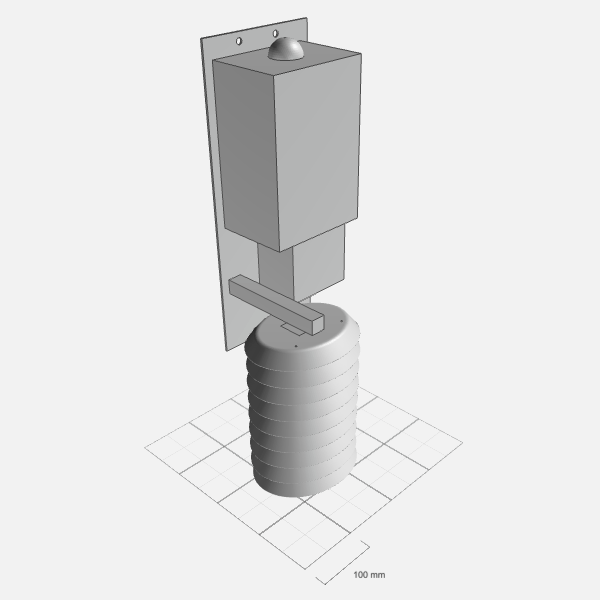
\includegraphics[width=6.5cm]
    {figures/utdNodeCropped.png}\label{fig:utdNode}

 \hfill \break
The UTD Node is a stationery sensor system consisting an array of IOT (Internet Of Things) sensors which is an extensible platform in which many newer sensors can be adopted into. The UTD Node houses a  particulate matter sensor, CO$_2$ sensor, climate sensor, a set of light sensors as well as an skyward facing camera. 

 \subsection*{2$^{nd}$ Generation: Central Nodes}
    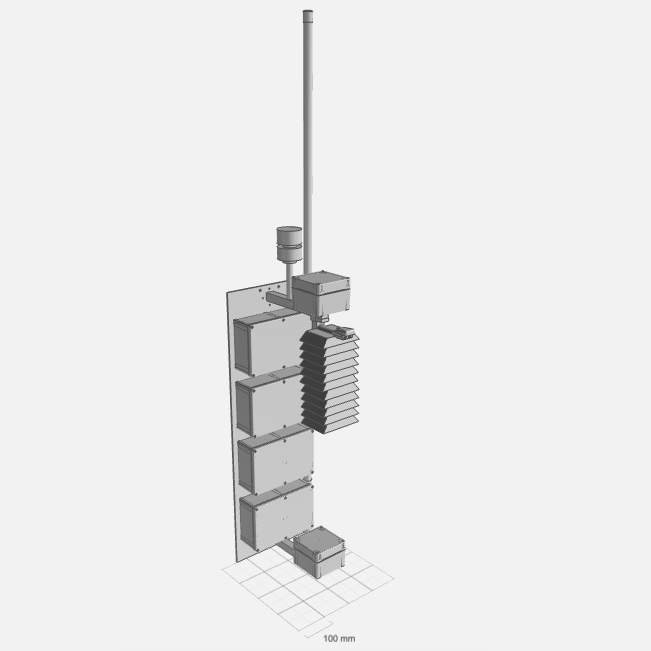
\includegraphics[width=6.5cm]
    {figures/centralNodeCropped.png}\label{fig:centralNode}
 \hfill \break
    
    Central Nodes are the second generation of UTD Nodes. In addition to providing all the sensors provided by the UTD Node, the Central Node has an expanded light sensing module as well as a radiation sensor, a sound sensor that detects bird calls as well as gunshots, a research grade ozone sensor, a lightning sensor, and remote power management capabilities. Additionally, the Central Node serves as a central gateway for a mesh network of LoRaWAN Nodes described in section \ref{subsubsec:loraWanNode}. 
    
 \subsubsection*{LoRaWAN Nodes}
 \label{subsubsec:loraWanNode}
    \includegraphics[width=6.5cm]
    {figures/loRaNodeV2Cropped.png}\label{fig:loranNode}
 \hfill \break
    LoRa is an infant communication technology based on ISM (Industrial, Scientific and Medical) bands which are capable of low power and Long Range applications. LoRaWAN is a Wide Area Network protocol that is designed to embed LoRa technology into a network infrastructure . The LoRa Nodes are designed to make use of LoRaWAN technology with each node a part of a mesh network communicating with one Central Node.

    The LoRa Nodes are designed to work without the need of direct power nor internet connectivity. This makes it extremely versatile. The main source of power for the LoRa Nodes is sunlight and thus it consists of two solar panels to harness solar energy.

    A LoRa Node consists of a particulate matter sensor and a climate sensor. 
     
\clearpage


\section*{Appendix D: \textbf{MINTS} GitHub repositories}
\begin{itemize}
      \item Version 1, 3 firmware:\\\url{https://github.com/mi3nts/minWeNodes}
      \item Version 4 firmware:\\\url{https://github.com/mi3nts/minWeZeroNodes}
      \item UTD Node firmware:\\\url{https://github.com/mi3nts/UTDNodes}
      \item Central Nodes firmware:\\\url{https://github.com/mi3nts/centralHub}
      \item LoRaWAN Nodes firmware:\\\url{https://github.com/mi3nts/LoRaWANNodes}
    \end{itemize}
\end{document}
